\documentclass[xcolor=dvipsnames]{beamer}
\mode<presentation>
{
	%agregar franja a lo largo del borde inferior de un slide que muestra el nombre del autor, el titulo de la presentacion, el numero del slide y otra informacion util ya que no viene por defecto. Debe ir antes de la definición del tema
	\useoutertheme{infolines}
	\usetheme[height=1cm]{Rochester} %opción especifica para el tema Rochester afecta a la franja superior
	\setbeamercovered{transparent} %las partes ocultas son transparentes en vez de invisible
	\usecolortheme[RGB={93,112,146}]{structure} %color global
}

% \pgfdeclareimage[height=1.2cm]{latex-logo}{logo-utal}
% \logo{\pgfuseimage{latex-logo}}

\usepackage{amssymb,amsmath}
\usepackage{multirow}
\usepackage{booktabs}
\usepackage{dcolumn}
\usepackage{rotating}
\usepackage{subfig}  %Subfloat

\usepackage[spanish]{babel}
\usepackage[utf8]{inputenc}
\usepackage{times}
\usepackage[T1]{fontenc}

\usepackage{listings}


\setbeamertemplate{blocks}[rounded][shadow=false] %cajas redondeadas y con sombra
\setbeamertemplate{navigation symbols}{}
\setbeamertemplate{caption}{\insertcaption} %solo el caption, sin anteceder la palabra Figura

\title[Trabajo de título]{Diseño e implementación del software de vuelo para un nano-satélite tipo cubesat}
\author[Carlos González Cortés]{
\footnotesize
Carlos González Cortés\\
\vspace*{1cm}
\textbf{Miembros de la comisión}\\
Dr. Marcos Díaz Quezada\\
Dr. Claudio Estévez Montero\\
Ing. Alex Díaz Becerra}
\date[Universidad de Chile]{}
\institute[]{Universidad de Chile}

\begin{document}

%% PORTADA %%
	\begin{frame}[plain]
        \begin{figure}[t]
            \begin{flushleft}
				
\includegraphics[scale=0.5]{img/logo.pdf}
            \end{flushleft}
        \end{figure}
        
		\titlepage
	\end{frame}

%% TABLA DE CONTENIDOS %%	
	\begin{frame}[shrink]
% 		\transdissolve
		\frametitle{Tabla de contenidos}
		\tableofcontents
	\end{frame}

%% INTRODUCCIÓN %%	
	\section{Introducción}
	\begin{frame}
% 		\transdissolve
		\frametitle{Introducción}
		
		\begin{block}{Proyecto SUCHAI}
		Diseño, construcción,  lanzamiento y operación de un nano-satélite, con fines educacionales y científicos.\\
		\vspace{0.3cm}
		\structure{Es el primer proyecto satelital desarrollado por estudiantes en el país.}
		\end{block}
		
		\begin{figure}[b]\centering
            \subfloat[Estandar Cubesat]{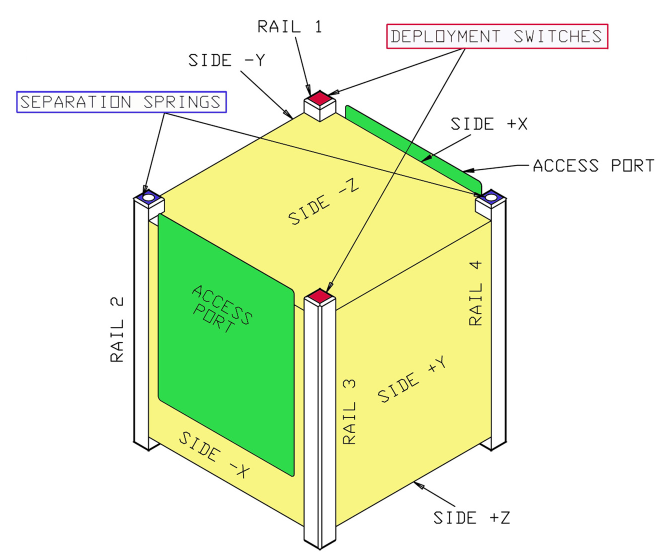
\includegraphics[height=0.5\textheight]{img/estandar.png}}
            \hspace{2cm}
            \subfloat[Cubesat SUCHAI]{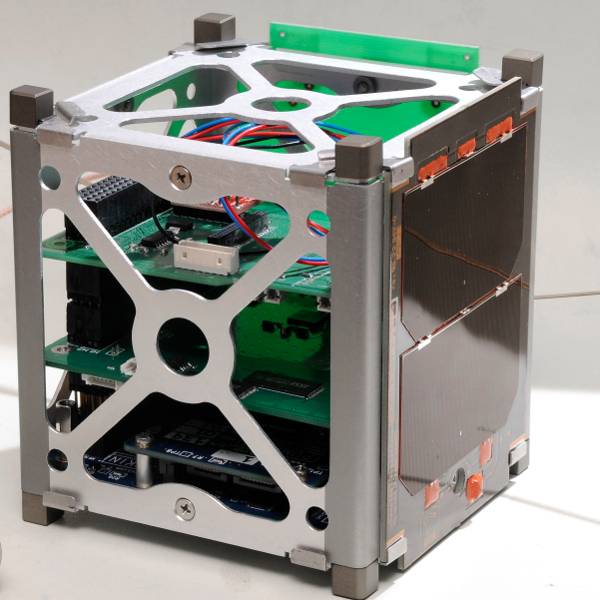
\includegraphics[height=0.5\textheight]{img/satelite.jpg}}
        \end{figure}
		
	\end{frame}
	
%% INTRODUCCIÓN %%
	\begin{frame}[squeeze]
        \frametitle{Introducción}
        \framesubtitle{Sistemas satelitales}
        \vspace{-0.5cm}
        \begin{figure}[t]\centering
            \subfloat[Subsistemas]{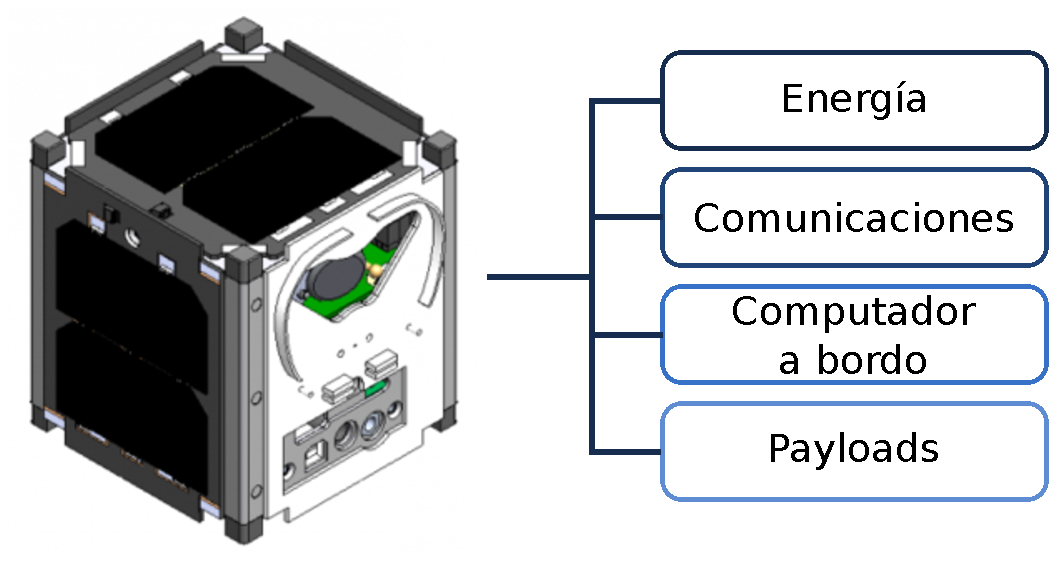
\includegraphics[height=0.4\textheight]{img/subsistemas.pdf}}
            \hspace{1cm}
            \subfloat[OBC]{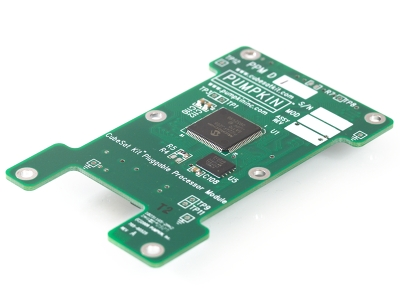
\includegraphics[height=0.4\textheight]{img/ppm.jpg}}
        \end{figure}
        
        \begin{block}{Computador a bordo}<+->
            Controla todas las operaciones del satélite e integra los diferentes subsistemas. Principales características:
            \begin{itemize}
                \item Microcontrolador PIC24F
                \item CPU @ 32 MHz
                \item Memoria RAM de 16 kB
                \item Memoria FLASH de 256 kB
            \end{itemize}
        \end{block}

    \end{frame}

%% OBJETIVOS %%
    \begin{frame}
        \frametitle{Introducción}
        \framesubtitle{Objetivos del trabajo}
        
        \begin{block}{Objetivos generales del trabajo}
            Diseñar e implementar el software que controla las operaciones del satélite una vez en órbita
        \end{block}
        
        \vspace{1cm}
        
        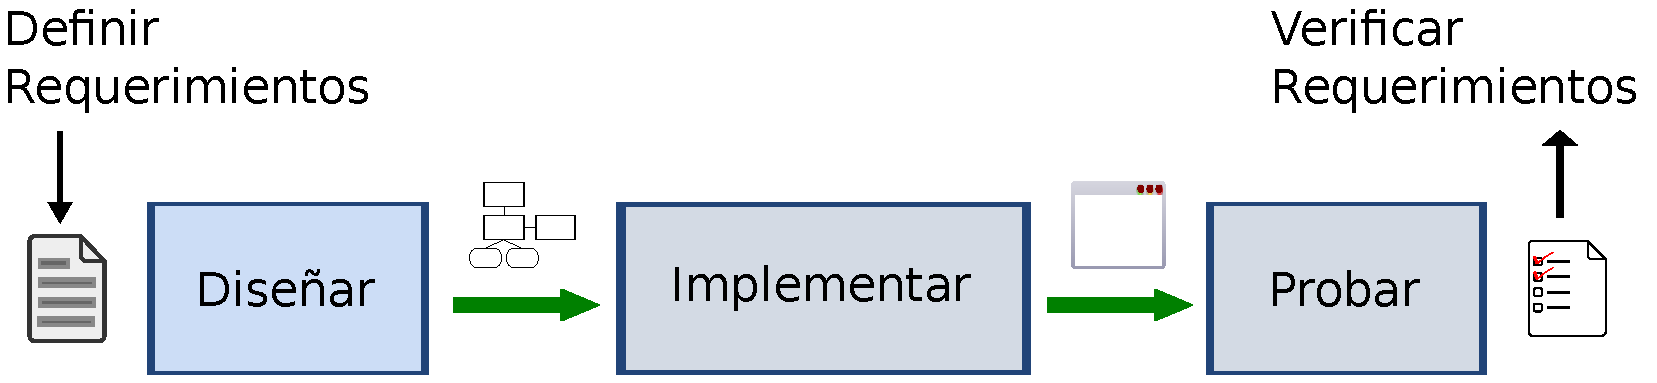
\includegraphics[width=0.99\textwidth]{img/objetivos.pdf}
        
    \end{frame}
    
%% MARCO TEORICO %%
    \section{Marco teórico}
    \subsection{Sistemas embebidos}
    \begin{frame}
        \frametitle{Marco teórico}
        \framesubtitle{Sistemas embebidos}
        
%         \begin{block}{Objetivos generales}<+->
        \begin{itemize}
            \item Diseñados para cumplir funciones específicas .
            \item Aplicaciones de tiempo real.
            \item Alto nivel de integración: CPU y periféricos
        \end{itemize}
        
        \vspace{0.5cm}
        \centering
        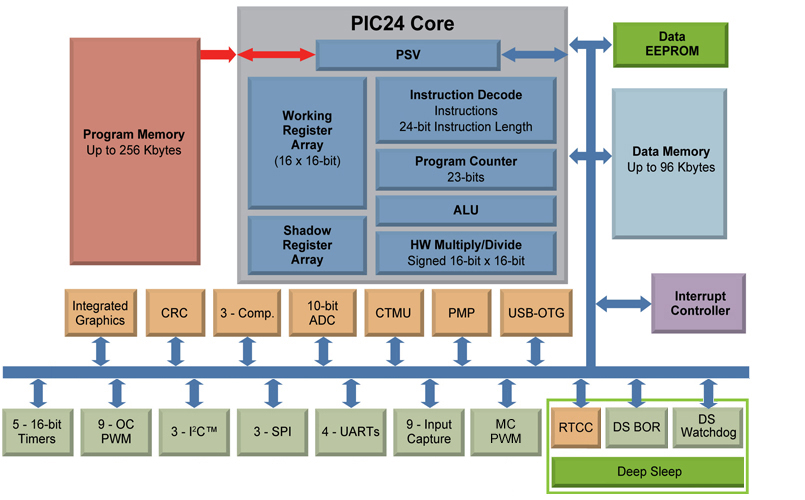
\includegraphics[scale=0.33]{img/pic_perif.jpg}
        
    \end{frame}
    
%% MARCO TEORICO %%
    \subsection{Sistemas operativos}
    \begin{frame}
        \frametitle{Marco teórico}
        \framesubtitle{Sistemas operativos}
        
            \begin{itemize}
                \item Sistemas operativos de tiempo real (RTOS)
                \begin{itemize}
                    \item Capa de abstracción entre la aplicación y el \textit{hardware}
                    \item Funcionan bajo requerimientos de \textit{timing} estrictos.
                    \item Deterministas en la ejecución de tareas.
                    \item Funcionamiento basado en eventos y prioridades.
                \end{itemize}
            \end{itemize}
            
        \vspace{0.5cm}
        \centering
        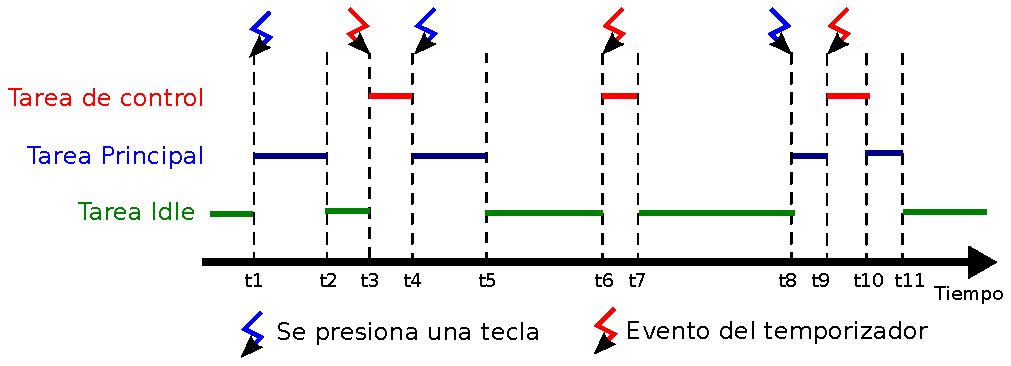
\includegraphics[width=0.99\textwidth]{img/rtos.pdf}
        
    \end{frame}
    
%% MARCO TEORICO %%
    \subsection{Patrones de diseño}
    \begin{frame}
        \frametitle{Marco teórico}
        \framesubtitle{Patrones de diseño}
        
        \begin{itemize}
            \item Técnica usada en desarrollo de software orientado a objetos.
            \item Soluciones bien probadas para cierto tipo de problemas.
            \item Patrón Procesador de Comandos.
            \begin{itemize}
                \item Separa la solicitud de una acción de su ejecución.
                \item Encapsula los requerimientos en comandos.
                \item Aplicaciones que soportan una gran cantidad de funciones.
            \end{itemize}

        \end{itemize}

        \vspace{0.3cm}
        \centering
        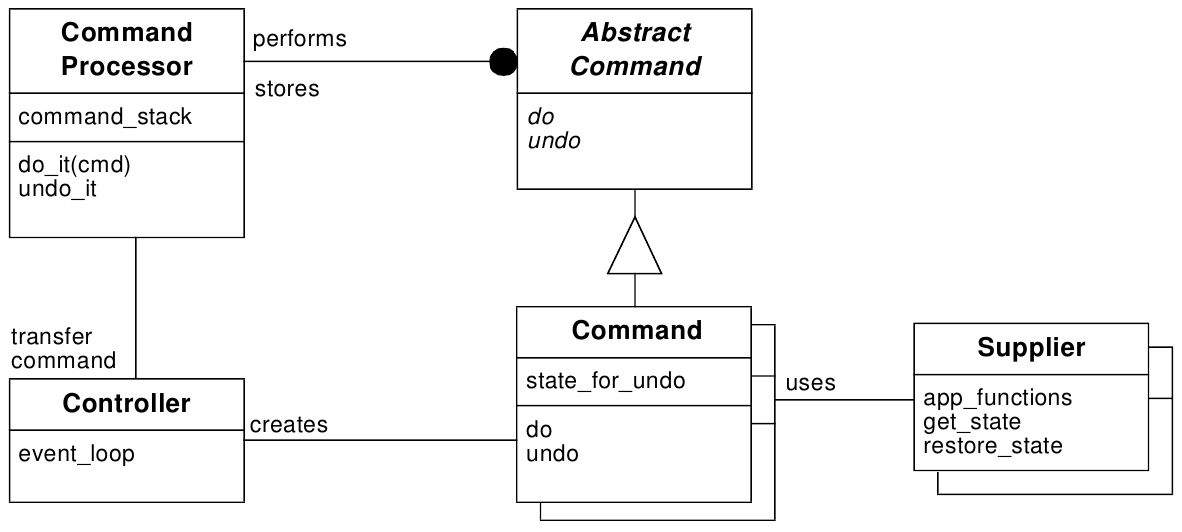
\includegraphics[height=0.6\textheight]{img/command_processor_class.png}
    \end{frame}
    
%% PROCESO DE DISEÑO %%
%     \section{Diseño}
%     \subsection{Requerimientos operacionales}
    \begin{frame}
%         \frametitle{}
%         \framesubtitle{}
%         \vspace{0.3\textheight}
        \centering \Large \structure{Proceso de diseño}
        
    \end{frame}
    
%% REQUERIMIENTOS OPERACIONALES %%
    \section{Diseño}
    \subsection{Requerimientos operacionales y no operacionales}
    \begin{frame}
        \frametitle{Diseño}
        \framesubtitle{Requerimientos operacionales}
        \centering
        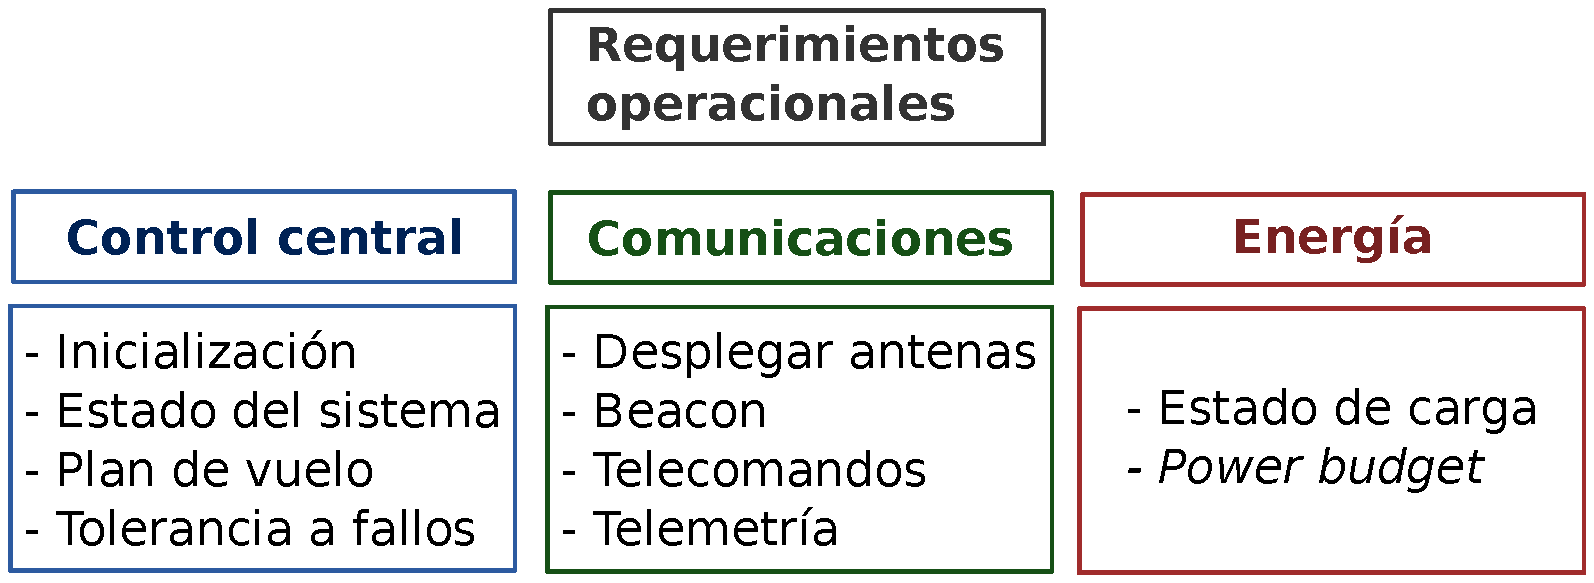
\includegraphics[height=0.45\textheight]{img/requerimientos_op.pdf}<+->
%         \vspace{0.5cm}
%         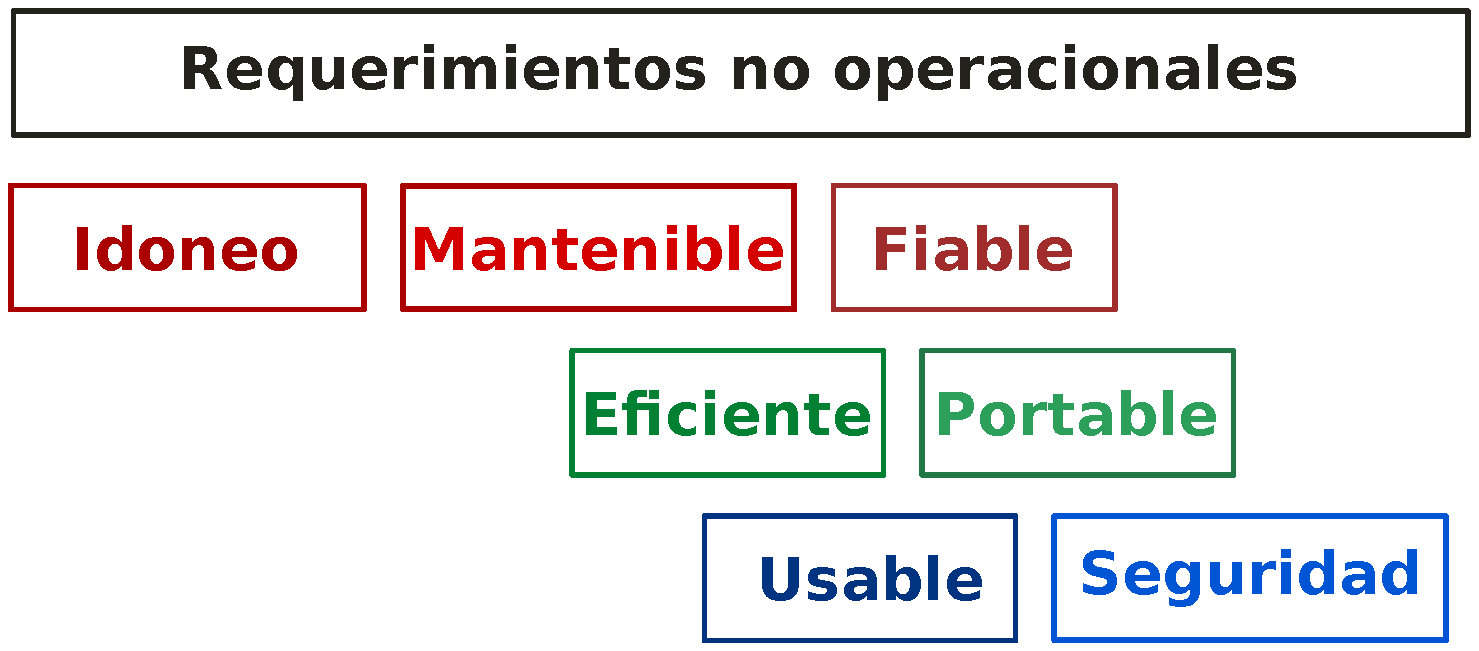
\includegraphics[height=0.40\textheight]{img/requerimientos_noop.pdf}<+->
    \end{frame}
    
%% REQUERIMIENTOS NO OPERACIONALES %%
%     \section{Diseño}
%     \subsection{Requerimientos operacionales}
    \begin{frame}
        \frametitle{Diseño}
        \framesubtitle{Requerimientos no operacionales}
        \centering
        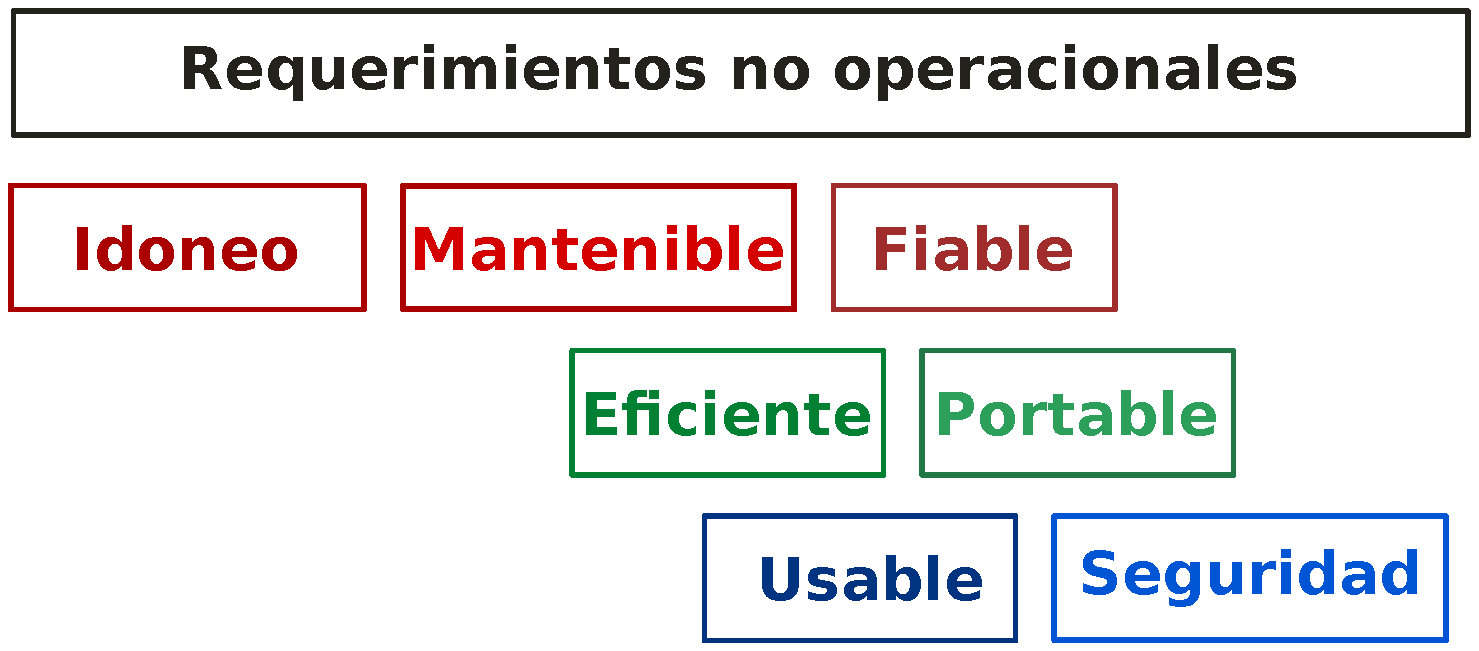
\includegraphics[height=0.45\textheight]{img/requerimientos_noop.pdf}
    \end{frame}

%% ARQUITECTURA GLOBAL %%
    \subsection{Arquitectura de software}
    \begin{frame}
        \frametitle{Diseño}
        \framesubtitle{Arquitectura global}
        
        \centering
        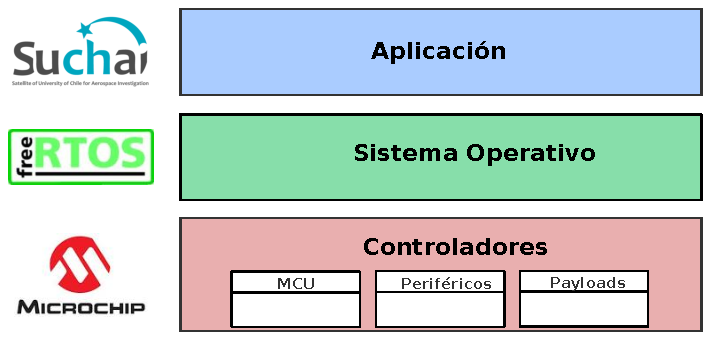
\includegraphics[width=0.99\textwidth]{img/arquitectura_global.pdf}

    \end{frame}
    
% %% ARQUITECTURA DRIVERS SISTEMA OPERATIVO %%
%     \subsection{Arquitectura controladores}
%     \subsection{Arquitectura sistema operativo}
%     \begin{frame}
%         \frametitle{Diseño}
%         \framesubtitle{Controladores y sistema operativo}
%         
%         \centering
%         \includegraphics[height=0.4\textheight]{img/arquitectura_controladores.pdf}
%         \vspace{0.5cm}
%         \includegraphics[height=0.5\textheight]{img/arquitectura_rtos.pdf}
%         
%     \end{frame}
    
%% ARQUITECTURA GLOBAL %%
%     \subsection{Arquitectura aplicación}
    \begin{frame}
        \frametitle{Diseño}
        \framesubtitle{Aplicación}
        
        \centering
        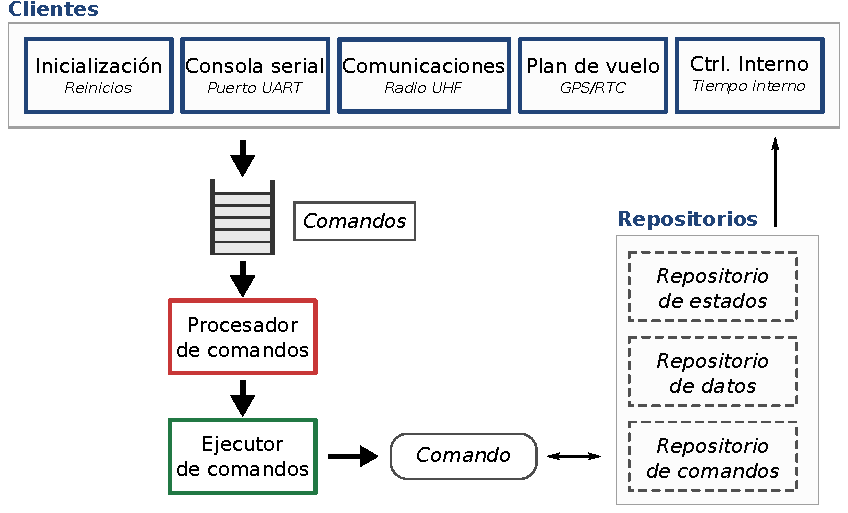
\includegraphics[width=0.99\textwidth]{img/arquitectura_suchai.pdf}
        
    \end{frame}
    
%% PROCESO DE IMPLEMENTACION %%
%     \section{Diseño}
%     \subsection{Requerimientos operacionales}
    \begin{frame}
%         \frametitle{}
%         \framesubtitle{}
%         \vspace{0.3\textheight}
        \centering \Large \structure{Proceso de implementación}
        
    \end{frame}
    
%% IMPLEMENTACION CLIENTES %%
    \section{Implementación}
    \subsection{Clientes}
    \begin{frame}
        \frametitle{Implementación}
        \framesubtitle{Clientes}

        \begin{itemize}
            \item Implementan la inteligencia del sistema.
            \item Tareas de FreeRTOS, concurrentes y de baja prioridad.
            \item Ejecución periódica, \textit{hard-realtime} o \textit{soft-realtime}.
        \end{itemize}
        
        \begin{center}
            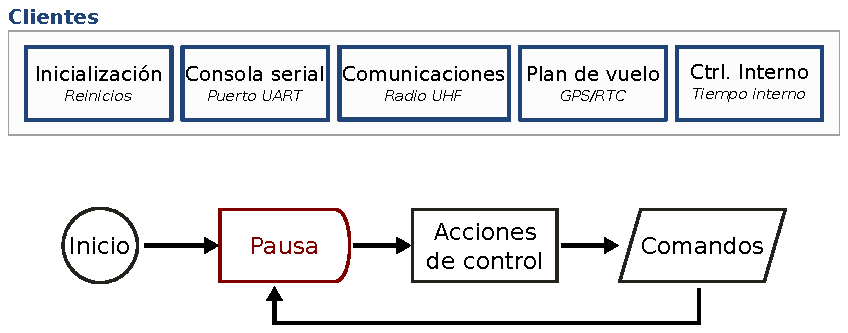
\includegraphics[width=0.99\textwidth]{img/implementacion_clientes.pdf}
        \end{center}
        
    \end{frame}
    
%% IMPLEMENTACION COMANDOS %%
    \subsection{Comandos}
    \begin{frame}
        \frametitle{Implementación}
        \framesubtitle{Comandos}
        
        \begin{itemize}
            \item Representados por estructura de datos.
            \item Se reconocen por su identificador y metadatos.
            \item Todo comando es una función.
        \end{itemize}
        
        \begin{center}
            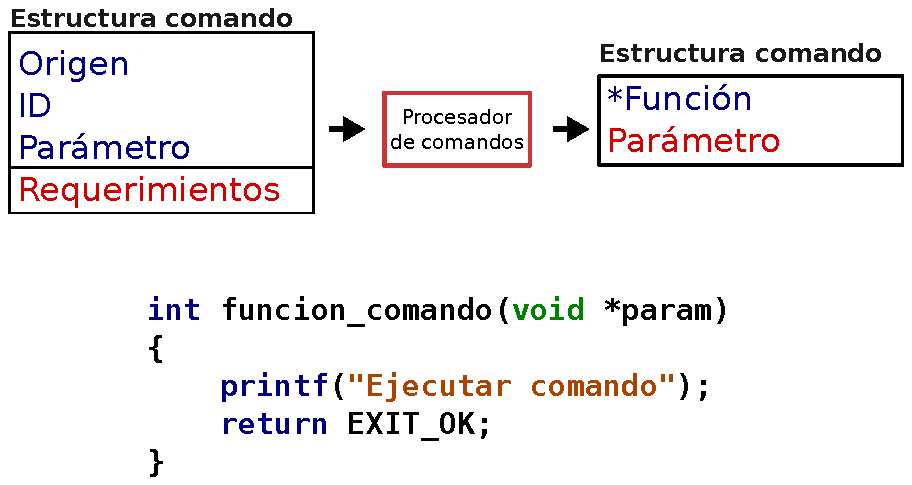
\includegraphics[width=0.8\textwidth]{img/implementacion_comandos.pdf}
        \end{center}
        
    \end{frame}
    
%% IMPLEMENTACION DISPATCHER-EXECUTER %%
    \subsection{Procesador de comandos}
    \begin{frame}
        \frametitle{Implementación}
        \framesubtitle{Procesador de comandos}
        
        \begin{itemize}
            \item Operaciones de control sobre comandos.
            \item Tareas de FreeRTOS, prioridad media.
            \item Ejecución basada en eventos.
        \end{itemize}
        
        \begin{center}
            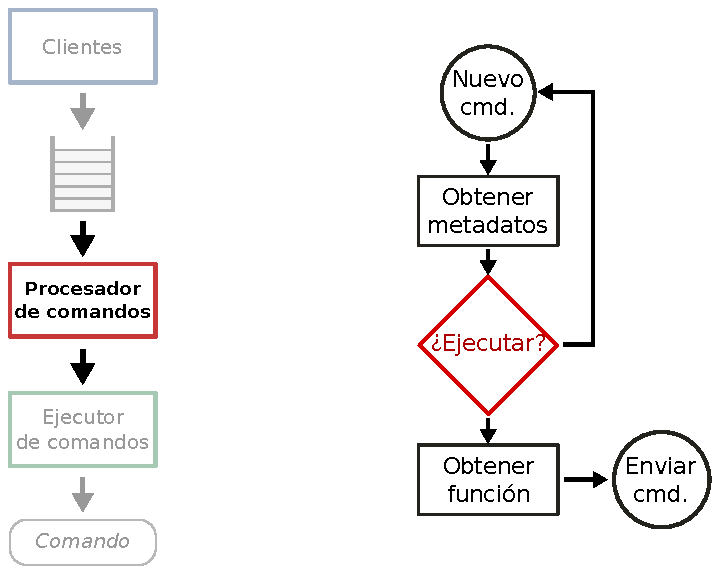
\includegraphics[height=0.75\textheight]{img/implementacion_dispatcher.pdf}
        \end{center}
        
    \end{frame}
    
%% IMPLEMENTACION DISPATCHER-EXECUTER %%
    \subsection{Ejecutor de comandos}
    \begin{frame}
        \frametitle{Implementación}
        \framesubtitle{Ejecutor de comandos}
        
        \begin{itemize}
            \item Entorno de ejecución para el comando.
            \item Tareas de FreeRTOS, alta prioridad.
            \item Ejecución basada en eventos.
        \end{itemize}
        
        \begin{center}
            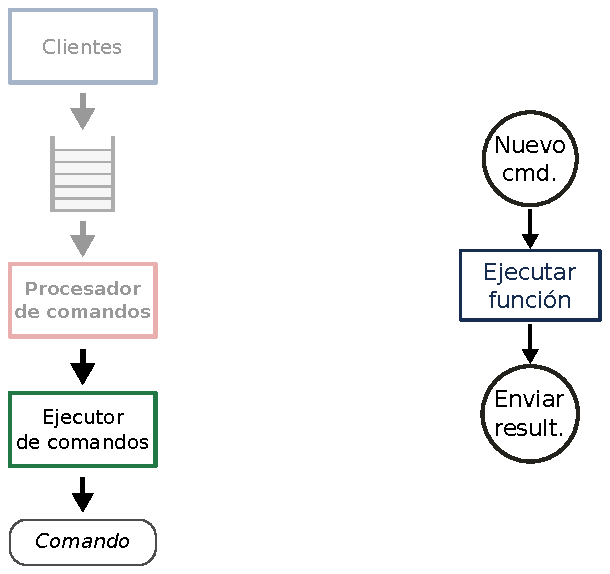
\includegraphics[height=0.75\textheight]{img/implementacion_executer.pdf}
        \end{center}
        
    \end{frame}
    
%% IMPLEMENTACION REPOSITORIOS %%
% \subsection{Ejecutor de comandos}
\begin{frame}
    \frametitle{Implementación}
    \framesubtitle{Repositorios}
    
    \begin{itemize}
        \item Librerías para manejo de datos.
        \item Lectura, escritura y gestión de diferentes tipos de información.
        \item Implementación requiere \textit{hardware} externo.
    \end{itemize}
    
    \begin{center}
        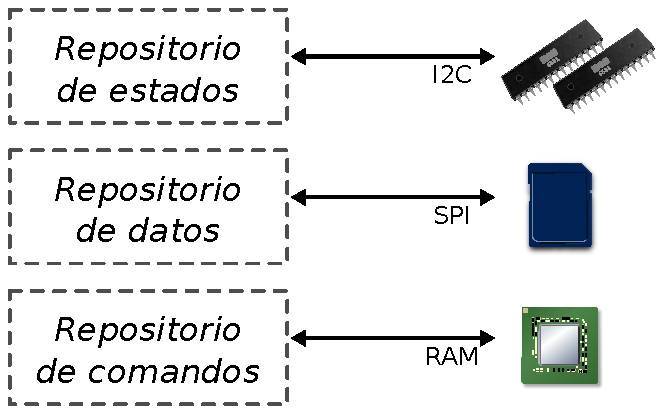
\includegraphics[height=0.5\textheight]{img/implementacion_repos.pdf}
    \end{center}
    
\end{frame}

%% PROCESO DE PRUEBAS %%
%     \section{Diseño}
%     \subsection{Requerimientos operacionales}
    \begin{frame}
%         \frametitle{}
%         \framesubtitle{}
%         \vspace{0.3\textheight}
        \centering \Large \structure{Pruebas y resultados}
        
    \end{frame}
    
%% PRUEBAS %%
%     \section{Pruebas}
%     \begin{frame}
%         \frametitle{Pruebas}
%         \framesubtitle{Pruebas de rendimiento}
%         \begin{center}
%             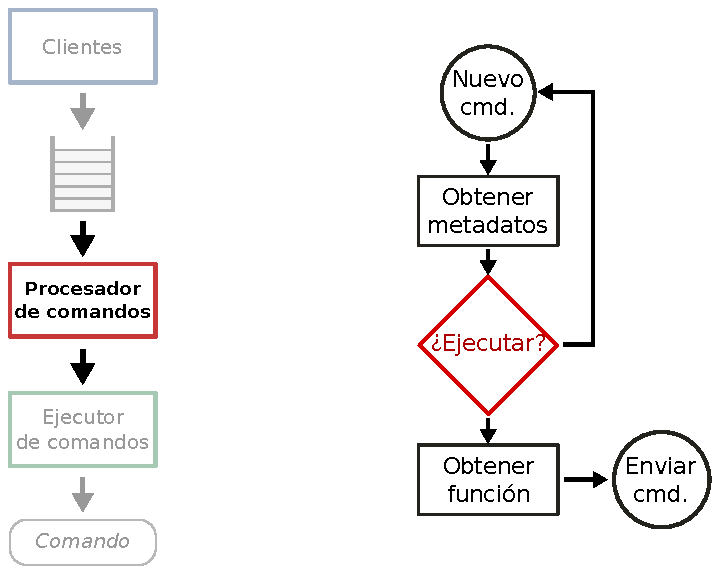
\includegraphics[height=0.99\textheight]{img/implementacion_dispatcher.pdf}
%         \end{center}
%         
%     \end{frame}
    
%% PRUEBAS %%
%     \section{Pruebas}
    \begin{frame}[squeeze]
        \frametitle{Pruebas}
        \framesubtitle{Verificación de requerimientos}
        
        \begin{itemize}
            \item \textit{Hardware in the loop simulation}
        \end{itemize}
        
        \begin{center}
            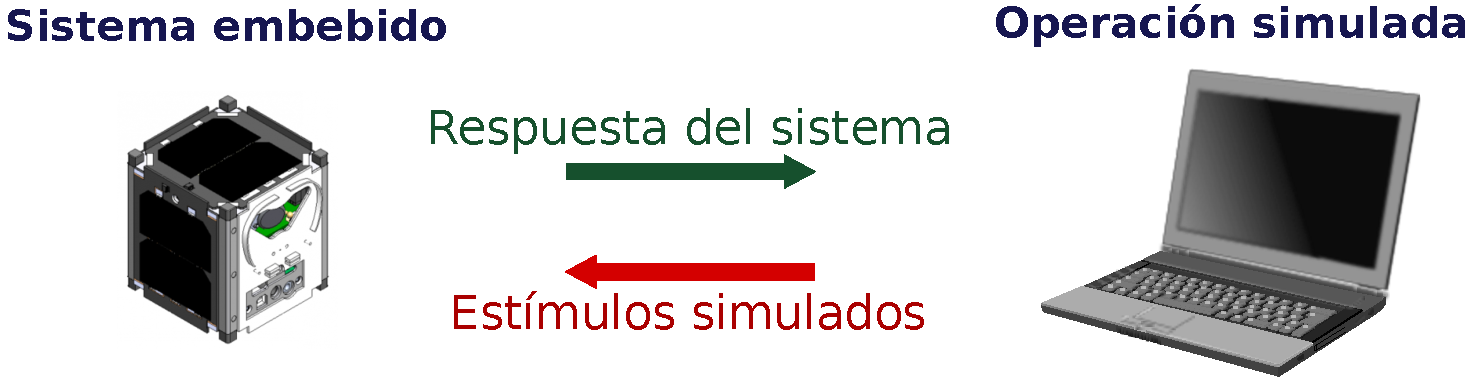
\includegraphics[height=0.3\textheight]{img/hil.pdf}
        \end{center}
        
        \begin{itemize}
            \item Montaje de la prueba
        \end{itemize}
        
        \begin{center}
            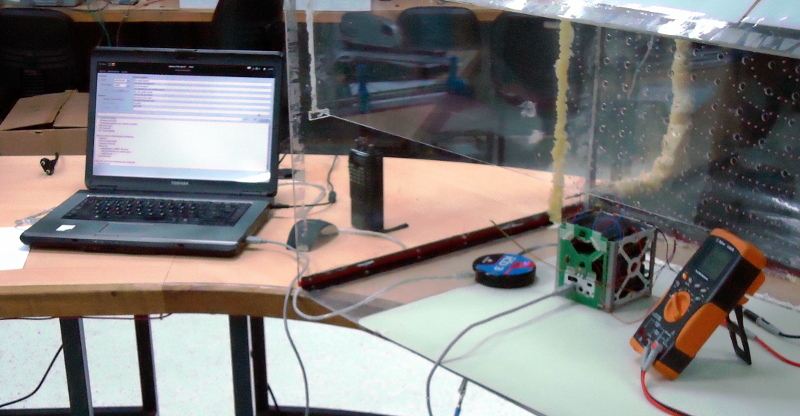
\includegraphics[height=0.45\textheight]{img/test_montaje.jpg}
        \end{center}
        
    \end{frame}

%% RESULTADOS CONTROL CENTRAL %%
    \section{Pruebas y resultados}
    \subsection{Control central}
    \begin{frame}[squeeze]
        \frametitle{Resultados}
        \framesubtitle{Control central}
        
        \begin{itemize}
            \item Inicio del sistema
                \begin{itemize}
                    \item Correcta inicialización de subsistemas.
                    \item Disponibilidad de consola serial para pruebas.
                \end{itemize}
            \item Plan de vuelo
            \begin{itemize}
                \item Se ejecuta un plan de vuelo con comandos cada 10 minutos.
                \item Se verifica la ejecución de los comandos.
            \end{itemize}
            \item Variables de estado
            \begin{itemize}
                \item Se registran las variables y se generan gráficos para verificación.
                \item Pruebas de reinicio y verificación de consistencia de variables.
            \end{itemize}
        \end{itemize}
        
        \begin{center}
            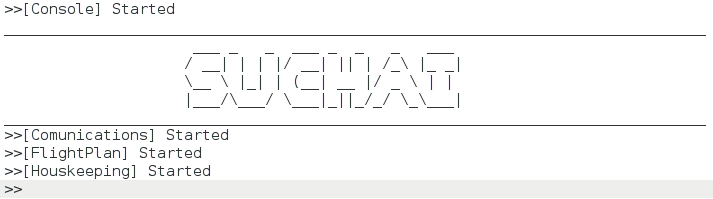
\includegraphics[height=0.35\textheight]{img/prompt.png}
        \end{center}

    \end{frame}
    
%% RESULTADOS ENERGIA %%
    \subsection{Energía}
    \begin{frame}
        \frametitle{Resultados}
        \framesubtitle{Energía}
        
        \begin{itemize}
            \item Estado de carga de baterías
            \begin{itemize}
                \item Se verifica la lectura de datos desde EPS.
                \item Se verifica la carga de la batería.
                \item Se verifica la estimación de SOC.
            \end{itemize}

            \item Presupuesto de energía
            \begin{itemize}
                \item Implementado en el procesador de comandos.
                \item Se simula operación con baja carga en baterías.
            \end{itemize}
            \item Resultados satisfactorios.
        \end{itemize}
                
        \small
        \begin{table}[b]
        \centering
        \begin{tabular}{llllll}
        \hline
        \textbf{Hora} & \textbf{Comando} & \textbf{SysReq} & \textbf{SOC} & \textbf{Resultado} \\ \hline
        20:18:33 & 0x300C &  4 & 4  & Ejecutado \\
        20:19:10 & 0x8000 & 10 & 4  & Rechazado \\
        20:19:13 & 0x8000 &  10 & 4  & Rechazado \\
        20:19:19 & 0x8002 &  10 & 4  & Rechazado \\
        20:19:19 & 0x5000 &  1 & 4  & Ejecutado \\
        20:19:45 & 0x8003 &  10 & 4  & Rechazado \\
        20:20:03 & 0x8003 &  10 & 4  & Rechazado \\ \hline
        \end{tabular} \label{ch5:table:test_soc}
        \end{table}

    \end{frame}
    
%% RESULTADOS COMUNICACIONES %%
    \subsection{Comunicaciones}
    \begin{frame}
        \frametitle{Resultados}
        \framesubtitle{Comunicaciones}
        
        \begin{itemize}
            \item Despliegue de antenas.
        \end{itemize}
        
        \begin{figure}[b]\centering
            \subfloat[Previo al despliegue]{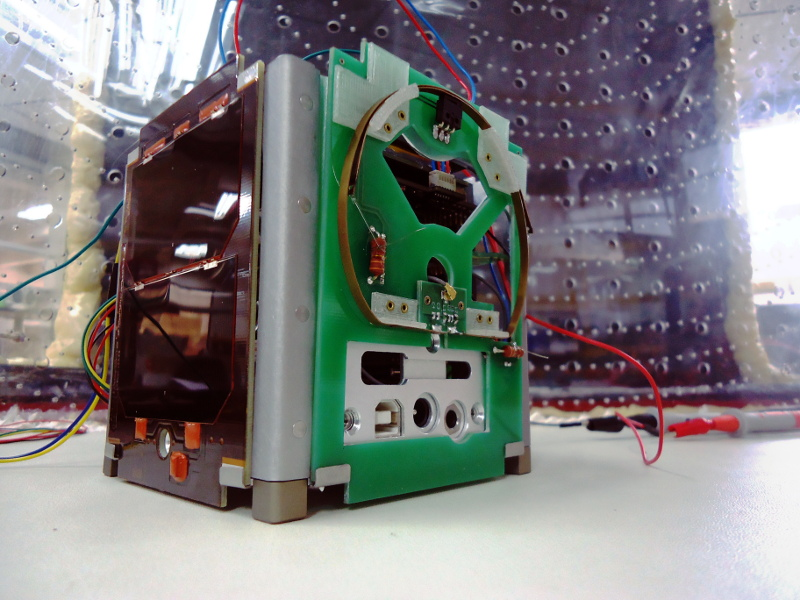
\includegraphics[width=0.45\textwidth]{img/test_deploy_pre.jpg}}
            \hspace{0.3cm}
            \subfloat[Antenas desplegadas]{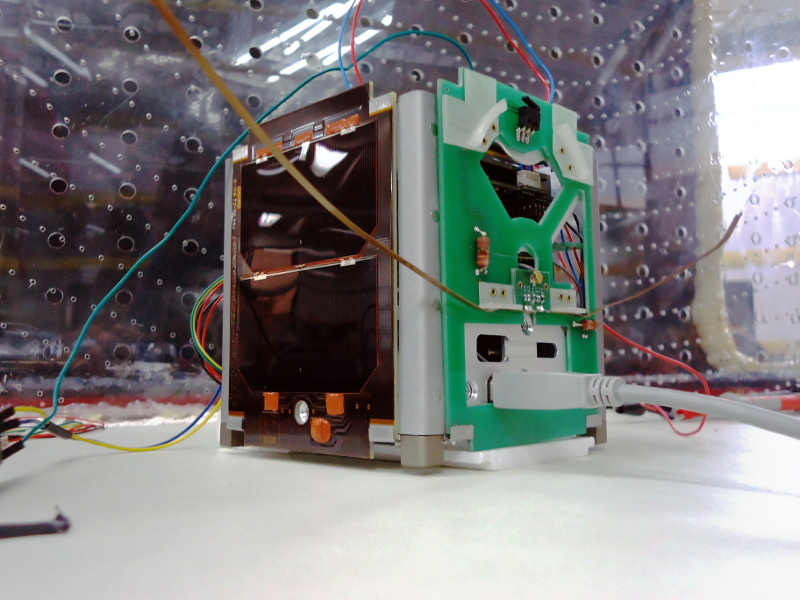
\includegraphics[width=0.45\textwidth]{img/test_deploy_post.jpg}}
        \end{figure}
        
    \end{frame}
        
    \begin{frame}
    \frametitle{Resultados}
    \framesubtitle{Comunicaciones}
        
        \begin{itemize}
            \item Generación, transmisión y recepción de \textit{beacons}.
            \begin{itemize}
                \item \texttt{SUCHAIATINGDOTUCHILEDOTCL-11000017H30761940780001}
                \item \texttt{00V0000000XHX02000000000000000GBW00000000DK000024}
            \end{itemize}
            \item Transmisión y recepción de telemetría y telecomandos.
            \item  \alert{Pruebas insatisfactorias}
        \end{itemize}

        \begin{figure}[b]\centering
            \subfloat[Recepción beacon]{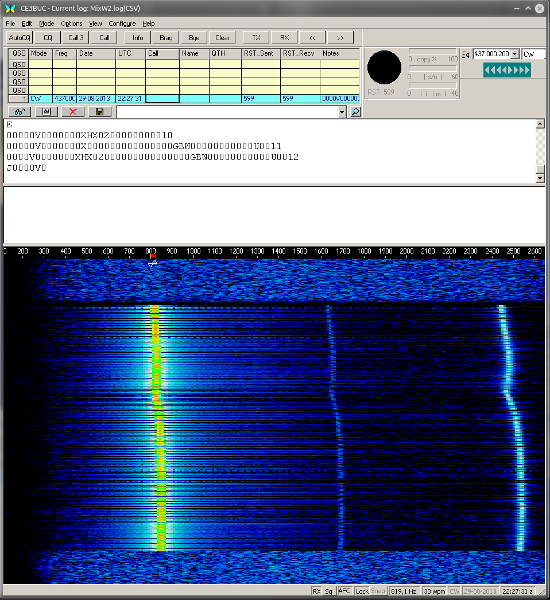
\includegraphics[height=0.55\textheight]{img/beacon2.png}}
            \hspace{0.5cm}
            \subfloat[Recepción telemetría]{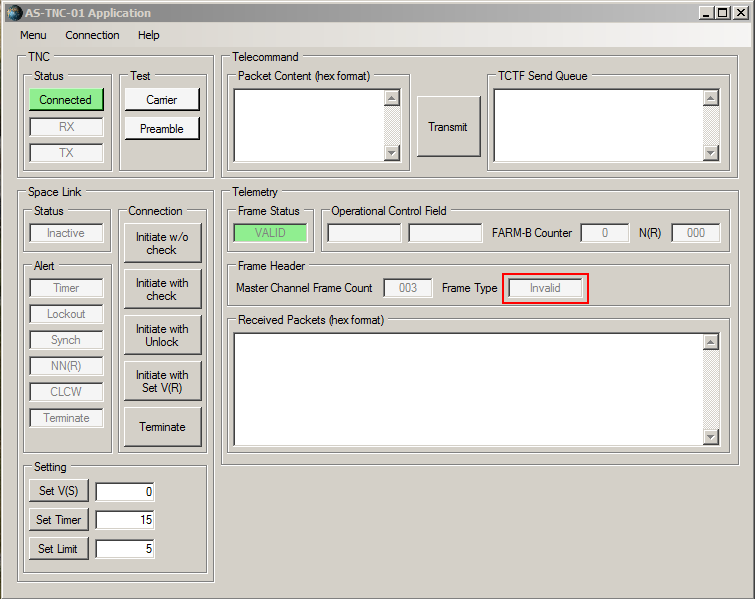
\includegraphics[height=0.55\textheight]{img/test_telemetria.png}}
        \end{figure}

    \end{frame}
    
%% PROCESO DE IMPLEMENTACION %%
%     \section{Diseño}
%     \subsection{Requerimientos operacionales}
    \begin{frame}
%         \frametitle{}
%         \framesubtitle{}
%         \vspace{0.3\textheight}
        \centering \Large \structure{Conclusiones}
        
    \end{frame}

%% CONCLUSIONES %%
    \section{Conclusiones}
    \begin{frame}
        \frametitle{Conclusiones}
%         \framesubtitle{Procesador y ejecutor de comandos}
        \begin{itemize}
            \item Uso generalizado de patrones de diseño, adaptados a lenguaje de programación procedural.
            \begin{itemize}
                \item Arquitectura de tres capas: divide el problema convenientemente.
                \item Procesador de comandos: permite cumplir con requerimientos operacionales y no operacionales.
            \end{itemize}
            
            \item FreeRTOS: una solución bien probada y robusta.
            \item Verificación de requerimientos.
            \begin{itemize}
                \item Se cumplen los requerimientos operacionales del área de control central, energía y \textit{payloads}
                \item No se cumplen los requerimientos del área de comunicaciones debido a fallas en el dispositivo.
            \end{itemize}
            \item Desarrollo de un proyecto de ingeniería, como parte del proceso de formación profesional: experiencia y desarrollo de habilidades blandas.

        \end{itemize}

    \end{frame}
    
%% TRABAJOS FUTUROS %%
%     \section{Trabajos futuros}
    \begin{frame}
        \frametitle{Trabajos futuros}
%         \framesubtitle{Procesador y ejecutor de comandos}
        \begin{itemize}
            \item Mejoras en el área de tolerancia a fallos.
            \item Agregar múltiples ejecutores de comandos.
            \item Portar el \textit{software} a diferentes plataformas.
            \item Integrar y probar un nuevo \textit{transceiver}.
        \end{itemize}

    \end{frame}
    
%% CONSULTAS %%
%     \section{Consultas}
    \begin{frame}
        \frametitle{Consultas}
%         \framesubtitle{Procesador y ejecutor de comandos}
        \centering
        \Large \structure{Muchas gracias por su atención}\\
        
        \normalsize \structure{¿Consultas?}\\
        
        \vspace{1cm}
        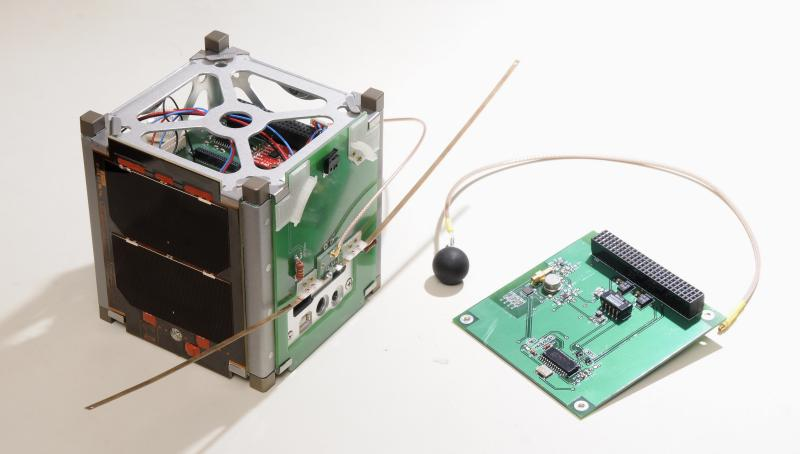
\includegraphics[width=0.7\textwidth]{img/suchai_satellite.jpg}
    \end{frame}
    
%% PROCESO DE IMPLEMENTACION %%
%     \section{Diseño}
%     \subsection{Requerimientos operacionales}
    \begin{frame}
%         \frametitle{}
%         \framesubtitle{}
%         \vspace{0.3\textheight}
        \centering \Large \structure{ANEXOS}
        
    \end{frame}
    
%% VARIABLES DE ESTADO %%
    \begin{frame}
        \frametitle{Variables de estado}
%         \framesubtitle{}
        \centering
        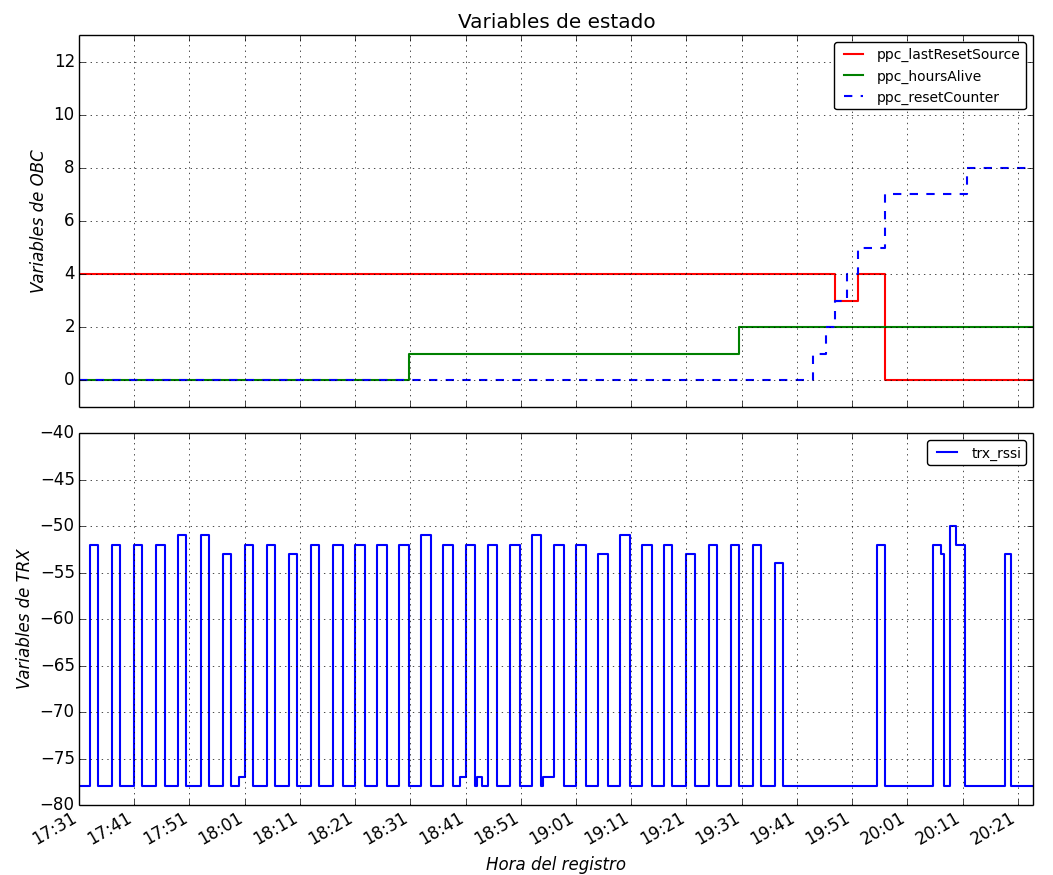
\includegraphics[height=0.99\textheight]{img/plot_status_var.png}
        
    \end{frame}
    
%% DATOS EPS %%
    \begin{frame}
        \frametitle{Variables EPS}
%         \framesubtitle{}
        \centering
        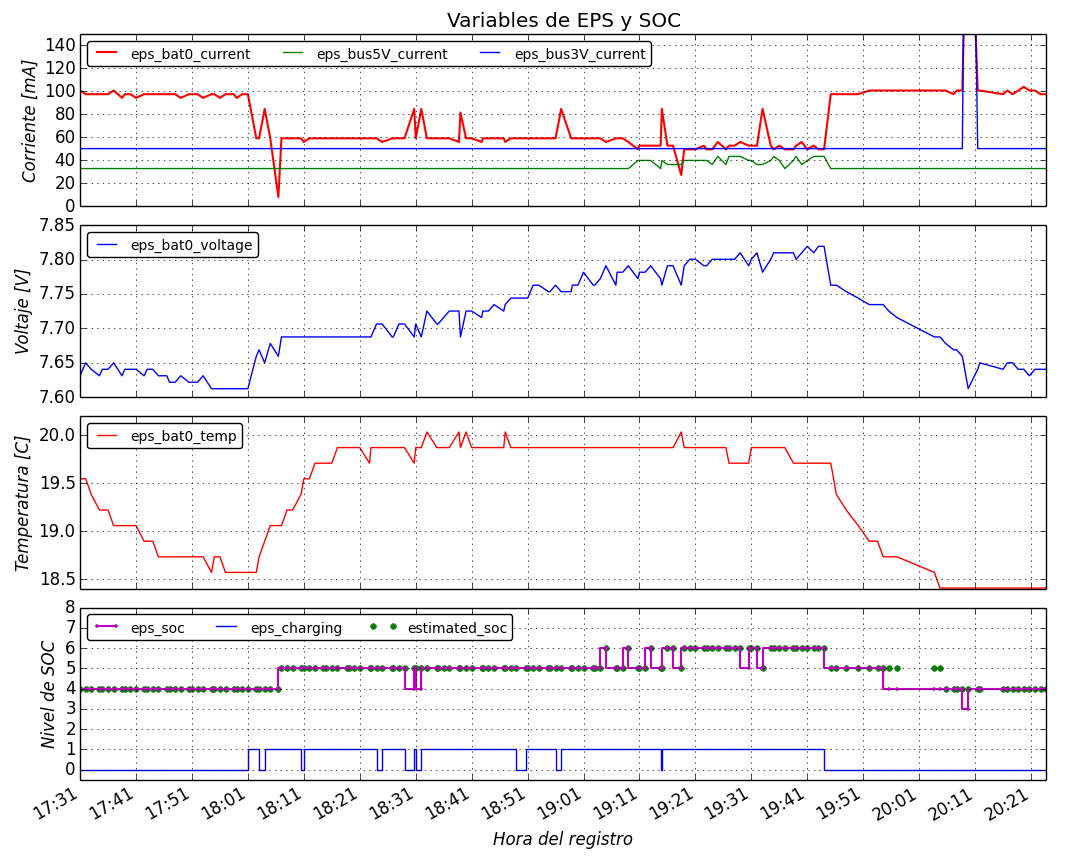
\includegraphics[height=0.99\textheight]{img/plot_soc.png}
        
    \end{frame}
    
%% DRIVERS %%
    \begin{frame}
        \frametitle{Drivers}
%         \framesubtitle{}
        \centering
        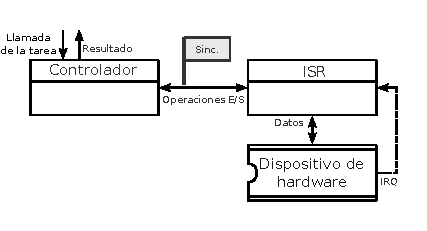
\includegraphics[height=0.3\textheight]{img/driver_sincrono.pdf}\\
        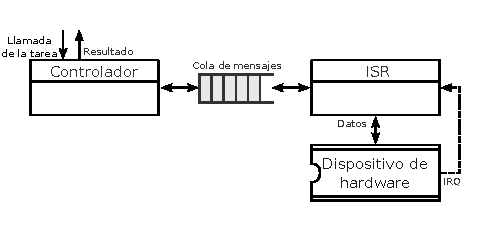
\includegraphics[height=0.3\textheight]{img/driver_asincrono.pdf}\\
        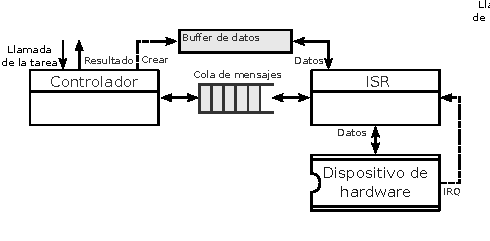
\includegraphics[height=0.3\textheight]{img/driver_serial.pdf}
    \end{frame}
    
%% DRIVERS %%
    \begin{frame}
        \frametitle{Calidad de software: ISO-25010}
%         \framesubtitle{}
        \centering
        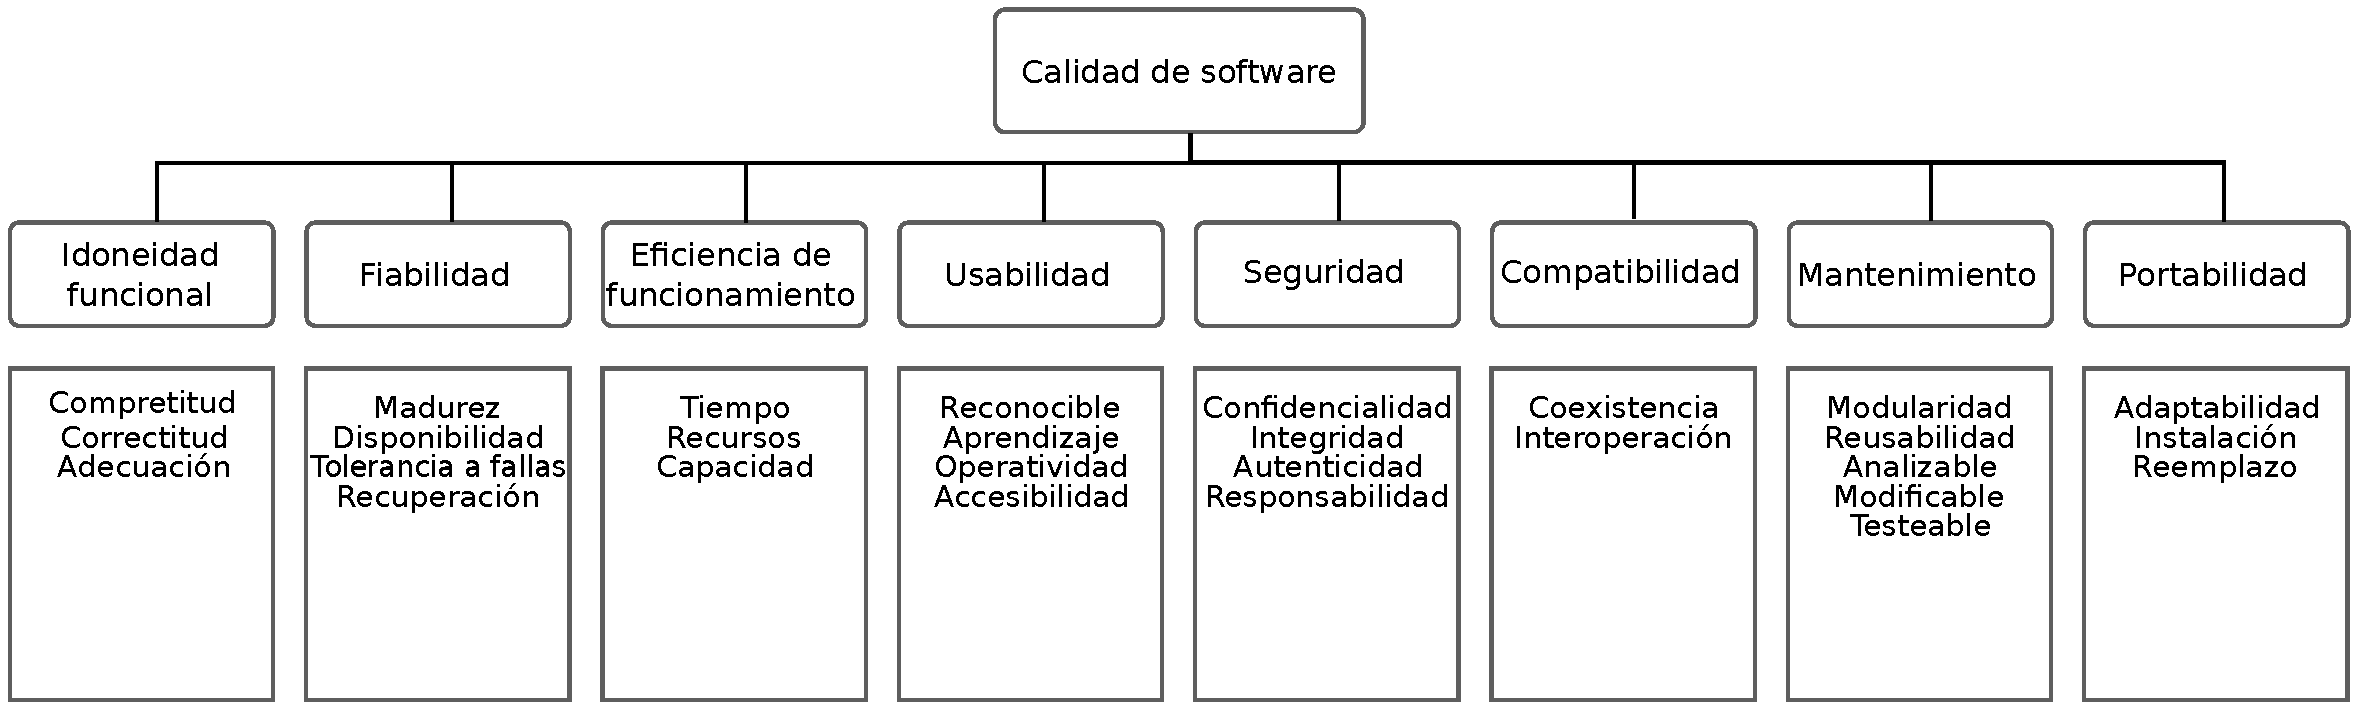
\includegraphics[width=0.99\textwidth]{img/ISO25010.pdf}\\
    \end{frame}
    
\end{document}
